% the sample slide is created with 16:9 aspect ratio
\documentclass[aspectratio=169,xcolor=dvipsnames]{beamer}

\usepackage{datetime2}
\DTMsetdatestyle{iso}

%\usepackage{xcolor}
\usepackage{forest}
\usepackage{adjustbox}
\usepackage{pgfgantt}


\ExplSyntaxOn
\NewDocumentCommand{\printrange}{m m}
{
	\int_eval:n { 1+#1*#2 } - \int_eval:n { (1+#1)*#2 }
}
\ExplSyntaxOff

% remove the options if you do not want to have them
\usetheme[
	% background=images/background.jpg, % you can add your own background image
	logo=images/unsw-portrait.png,
	sidelogo=images/unsw-landscape.png,
]{unsw}
% uncomment to show notes. Works very nicely with dspdfviewer. You get something similar to PPT's presenter view.
%\usepackage{pgfpages}
%\setbeameroption{show notes on second screen}

% information for the title page
\author{Samuel Marks, PhD}
\title{Multi-ML cross-platform\\meta-programming at scale}
\def\myTitle{Multi-ML cross-platform meta-programming at scale}
\subtitle{using compiler tech and C}
\institute{Computer Science Engineering}

\date{Annual review \today}

\begin{document}
% use plain option to remove the page number from the title slide
\begin{frame}[plain]
	\titlepage
\end{frame}

\begin{frame}{Introduction}
	\textbf{Programming solutions}\\
	Nothing I build will be popular. Neither a new language nor a new framework. Thus, rather than attempt to solve problems of dev speed, scale and quality this way; these are solved through automated interoperability.\vspace{1em}

	\textbf{Deployment (multicloud, DevOps)}\\
	Deploying software is complicated by the multitude of cloud vendors, operating systems, and depth of dependencies; including databases and libraries.\vspace{1em}

	\textbf{Fractionated ML}\\
	The ML field is moving too rapidly. There is little confidence to be found in SOTA claims (e.g., in medicine).
\end{frame}

\begin{frame}{Biography}
	\framesubtitle{Samuel Marks}
	\begin{block}{Academic}
		Holds PhD from the University of Sydney.
	\end{block}

	\begin{exampleblock}{Commercial}
		Delivered many dozens of projects for dozens of companies over 10+ years.
	\end{exampleblock}

	\begin{alertblock}{Charitable}
		Working on facilitating mass screening programmes for blinding eye diseases.
	\end{alertblock}
\end{frame}

\begin{frame}{History and definitions}
	Open thesis PDF
\end{frame}

\pgfkeys{/pgf/inner sep=0.24em}
\begin{frame}
	\begin{forest} for tree={grow'=0,anchor=west,child anchor=west},
		[\textbf{Degrees of Freedom I}
				[OS,for tree={fill=MidnightBlue,text=white}
						[Microsoft,for tree={fill=yellow,text=black}
								[Windows]
								[DOS]]
						[\textellipsis{}]
						[Linux]
						[Mobile,for tree={fill=Emerald,text=white}
								[Android]
								[iOS]]]
				[Architecture,for tree={fill=Sepia,text=white}
						[Embedded,for tree={fill=Mahogany}]
						[Networked,for tree={fill=RawSienna}
								[Peer-to-peer]
								[Client/server, for tree={}
										[Single]
										[Master/slave]
										[Consensus]]]]
				[Language,for tree={fill=black,text=white}
						[C,for tree={}]
						[TypeScript,for tree={}]
						[Swift,for tree={}]
						[\textellipsis{}]
						[Python,for tree={}]]]
	\end{forest}
\end{frame}

\begin{frame}
	\begin{forest} for tree={grow'=0,anchor=west,child anchor=west},
		[\textbf{Degrees of Freedom II}
				[ML,for tree={fill=BlueViolet,text=white}
						[Framework,for tree={}
								[CNN]
								[RNN]
								[Transformers]
								[Gradient boosting]
								[\textellipsis{}
									[Optimiser[Learning rate][\(\alpha\)][\textellipsis{}]]
									[\textellipsis{}]
									[Loss]]
								[Ensembles]
								[Multimodal]]]
				[Cloud,for tree={fill=BurntOrange,text=white}
						[Amazon Web Service (AWS)]
						[Google Cloud]
						[\textellipsis{}]]]
	\end{forest}
\end{frame}

\part[foo]{bar}

\begin{frame}
	\begin{forest} for tree={grow'=0,anchor=west,child anchor=west}, [\textbf{D of F III}
				[Codebases,for tree={fill=MidnightBlue,text=white}
						[Databases,for tree={fill=ForestGreen,text=white}]
						[Languages,for tree={fill=Emerald,text=white}
								[Frontend]
								[Backend]]]
				[Users,for tree={fill=Sepia,text=white}
						[one server,for tree={fill=BrickRed}]
						[\textgreater{} one server,for tree={fill=Melon,text=black}]]
				[Stakeholders,for tree={fill=black,text=white}
						[\textellipsis{},for tree={fill=gray}]
						[Teams,for tree={fill=BlueViolet,text=white}
								[Non-Developers,for tree={fill=YellowOrange,text=black}
										[Analytics]
										[Documentation]]
								[Developers,for tree={fill=Bittersweet}
										[Codebase quality,for tree={}
												[Tests]
												[\textellipsis{}]
												[Docs]]
										[Codebase interoperability]]]]]
	\end{forest}
\end{frame}

\begin{frame}{Thesis ontology}
	\begin{forest} baseline,for tree=draw
		[\textbf{\myTitle}[Compilers,for tree={fill=MidnightBlue,text=white}[C,for tree={fill=yellow,text=black}[Multicloud][FFI; wrap; package]][\(\ldots\)][TypeScript][Python,for tree={fill=Emerald,text=white}[Multi-ML]]][Multiarch,for tree={fill=Sepia,text=white}[Consensus,for tree={fill=Mahogany}][Networking,for tree={fill=RawSienna}]]]
	\end{forest}
\end{frame}

\begin{frame}{Interoperability}
	\begin{quote}
		The ability of two or more systems or components to exchange information and to use the information that has been exchanged.
		\\{\normalfont --- IEEE Standard Computer Dictionary (1990)}
	\end{quote}

	Aside from using same language [runtime], networking, and executable chains; there are two basic ways of achieving interoperability:
	\vspace{1em}
	\begin{columns}[t]
		\begin{column}[T]{0.4\textwidth}
			\textbf{DSL (types)}\hskip 1.705cm \textbf{DSL (API)}\\
			\begin{columns}[t]
				\begin{column}[T]{0.807\textwidth}
					\begin{itemize}
						\item IDL (1983)
						\item ASN.1 (1984)
						\item SGML (1986)
						\item XML Schema (2001)
						\item JSON Schema (2009)
						\item \textellipsis{}
					\end{itemize}
				\end{column}
				\begin{column}[T]{0.7\textwidth}
					\begin{itemize}
						\item SOAP (1998)
						\item WSDL (2000)
						\item WADL (2009)
						\item OpenAPI (2011)
						\item AsyncAPI (2016)
						\item \textellipsis{}
					\end{itemize}
				\end{column}
			\end{columns}
		\end{column}
		\begin{column}[T]{0.4\textwidth}
			\hskip 1cm \textbf{C}\\
			\begin{itemize}
				\item \texttt{extern} to embed within C++
				\item Binary level
				\item Library level
				\item ABI
				\item FFI for most every other language
			\end{itemize}
		\end{column}
	\end{columns}
\end{frame}

\forestset{box/.style={
draw, no edge, l=0, l sep=1.5ex,
calign=first, anchor=base west,
content format={\strut\forestoption{content}},
if n children=0{}{
after packing node={
minimum width/.pgfmath=
	{s("!l")+max_x("!l")-s("!1")-min_x("!1")}, % 43
for children/.wrap pgfmath arg={s+={##1}}{0},
typeset node}}}}
\begin{frame}{Languages and targets \(\dfrac{I}{II}\)}
	\begin{forest}
		for tree={box} [Native
			[Mobile
					[iOS[Swift]]
					[Android[Kotlin][Java]]]
			[Desktop
					[macOS[Python]]
					[Linux[Rust]]
					[Windows[\textellipsis{}]]
					[*BSD]
					[SunOS]]]
	\end{forest}
\end{frame}

\begin{frame}{Languages and targets \(\dfrac{II}{II}\)}
	\begin{forest}
		for tree={box} [Browser
			[Web
					[WASM[C]]
					[Traditional[TypeScript]]]]
	\end{forest}
	\(\leftarrow\) all 7 can target any OS (except Swift on Android, and Java on iOS)
\end{frame}

\begin{frame}{C}
	A popular programming language invented in 1972. With support across:
	\begin{columns}[t]
		\begin{column}[T]{0.4\textwidth}
			\textbf{Operating Systems}
			\vspace{1em}
			\begin{columns}[t]
				\begin{column}[T]{0.416\textwidth}
					\begin{itemize}
						\item Android
						\item iOS
						\item Linux
						\item Windows
						\item DOS
					\end{itemize}
				\end{column}
				\begin{column}[T]{0.4\textwidth}
					\begin{itemize}
						\item web
						\item macOS
						\item SunOS
						\item *BSD
						\item \textellipsis{}
					\end{itemize}
				\end{column}
			\end{columns}
		\end{column}
		\begin{column}[T]{0.4\textwidth}
			\textbf{Programming Languages}
			Foreign Function Interfaces
			\begin{columns}[t]
				\begin{column}[T]{0.4\textwidth}
					\begin{itemize}
						\item Python
						\item Rust
						\item Swift
						\item PHP
						\item Crystal
					\end{itemize}
				\end{column}
				\begin{column}[T]{0.4\textwidth}
					\begin{itemize}
						\item Java
						\item Erlang
						\item Haskell
						\item Nim
						\item \textellipsis{}
					\end{itemize}
				\end{column}
			\end{columns}
		\end{column}
	\end{columns}
\end{frame}

\begin{frame}{Multi-ML}
	NOTE: The landscape is changing. I am a top 10 contributor to Google's [TensorFlow] Keras. A month ago they released a cross-compatible version that makes interchangeable PyTorch, JAX, and TensorFlow.
\end{frame}

\begin{frame}{Multi-ML}
	There are ~10 commonly used ML frameworks. Each have different ecosystems, and when a new research paper---or industry project---is released, they (usually) target just one framework.\vspace{1em}

	My new multi-ML framework is created by applying my \texttt{cdd-python} compiler to 10 different popular ML frameworks (at the source-code level). This exposes CLIs, REST APIs, database tables and other useful layers.\vspace{1em}

	Now, given a problem (e.g., determine best dataset for my new optimiser, or determine best [AUCROC] model for my new dataset), the framework will optimise across a \textit{search space} traversing permutations of parameters (e.g., optimiser, loss function) and hyperparameters (e.g, \(\alpha\), \(\beta\), learning rate). Where \textit{search space} can include everything that the ML ecosystem has to offer.
\end{frame}

{
\usebackgroundtemplate{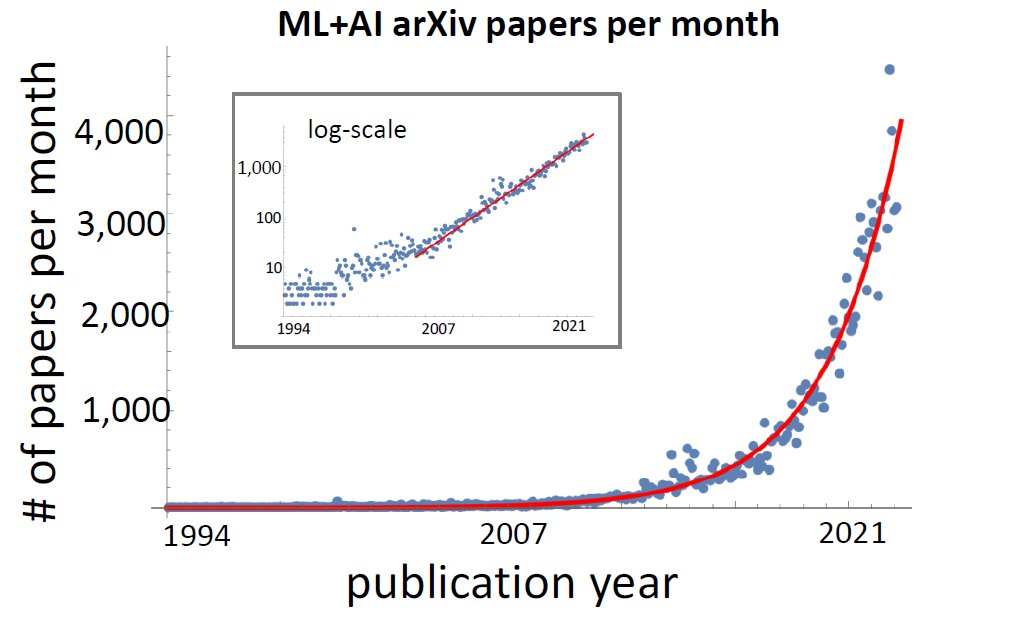
\includegraphics[width=\paperwidth]{images/number_of_AI_papers_on_arXiv_per_month.jpg}}
\begin{frame}[plain]
\end{frame}
}

\begin{frame}{Multi-ML - Future work \(\dfrac{I}{II}\) (post-PhD; or by others)}
	Take arbitrary repos with Python packages or simple Notebooks \& automatically:

	\begin{enumerate}
		\item[0.] Find and clone candidate repositories (e.g., from the arXiv);
		\item Make OS independent;
		\item Remove absolute paths (e.g., to weight files);
		\item Format and autolint;
		\item Add type hints;
		\item Separate steps to be compatible with ensemble use-cases, e.g., move the model construction to its own function, and constants [like kernel sizes] to a consistent section;
		\item Send pull-request / merge-request to repository;
		\item If PR is accepted, add new model, optimizer, loss function, or other relevant `thing' to this multi-ML meta-framework's search-space;
		\item Publish (online) benchmarks of this new `thing' against similar `thing's on a variety of different datasets.
	\end{enumerate}
\end{frame}

\begin{frame}{Multi-ML - Future work \(\dfrac{II}{II}\) (post-PhD; or by others)}
	\begin{enumerate}
		\item[0.] Automatically systematically review articles [with public datasets] coming through different research fields;
		\item run their claims against the entire search-space of this multi-ML meta-framework;
		\item (if improvement detected) write up a research paper with a new claim.
		\item (if improvement detected) Open-source the (new) result with clear replication steps.
	\end{enumerate}
	\vspace{2em}

	\begin{columns}
		\begin{column}[T]{0.4\textwidth}
			Add support for new ML frameworks.
		\end{column}
		\begin{column}[T]{0.4\textwidth}
			Analytics and dashboarding.
		\end{column}
	\end{columns}
\end{frame}


\begin{frame}{Multiclustering}
	Depending on ones use case, different architectures make sense, commonly they are:
	\begin{itemize}
		\item Embedded
		\item Client/server
		      \begin{itemize}
			      \item Single server
			      \item Master/slave
			      \item Consensus
			            \begin{itemize}
				            \item One master multiple slaves
				            \item Read-only slaves with multiple masters
				            \item Peer-to-peer
			            \end{itemize}
		      \end{itemize}
	\end{itemize}

	Focussing on multiclustering means not ignoring the scalability problems of software-engineering. Implementation TBD, and to be authored in C.
\end{frame}

\begin{frame}{Multicloud and DevOps}
	There are a large number of cloud vendors with an exponentially larger number of DevOps tooling. Both complicate software development, maintenance, compliance, security, and debugging.\vspace{1em}

	\begin{columns}[t]
		\begin{column}[T]{0.4\textwidth}
			\textbf{Multicloud}\\
			Created new cloud vendor client libraries in C. With focus on FFI interoperability and cross-platform compatibility, these can be called on any system and by any language or extensible framework.
		\end{column}
		\begin{column}[T]{0.4\textwidth}
			\textbf{DevOps}\\
			Portable cross-platform single application version managers are developed. Each can run in any configuration management tool (25+) and on any OS; and thus any cloud.
		\end{column}
	\end{columns}
\end{frame}

% \begin{frame}{Progress Graphic}
% \end{frame}

% \begin{frame}{Summary}
% \end{frame}

\begin{frame}{Future work}
	We can also add two columns in the slides.
	\begin{columns}[t]
		\begin{column}[T]{0.4\textwidth}
			Instrument compilers to trans bodies
			\vspace{1em}
		\end{column}
		\begin{column}[T]{0.4\textwidth}
			Auto read/write papers, replicate their result then improve [Multi-ML] then publish (all automatic)
		\end{column}
	\end{columns}
\end{frame}

\begin{frame}{Plan \(\dfrac{I}{III}\)}
	\begin{adjustbox}{max totalsize={1.1\textwidth}{\textheight},center}
		\definecolor{barblue}{RGB}{153,204,254}
		\definecolor{groupblue}{RGB}{51,102,254}
		\definecolor{linkred}{RGB}{165,0,33}
		\renewcommand\sfdefault{phv}
		\renewcommand\mddefault{mc}
		\renewcommand\bfdefault{bc}
		\setganttlinklabel{s-s}{START-TO-START}
		\setganttlinklabel{f-s}{FINISH-TO-START}
		\setganttlinklabel{f-f}{FINISH-TO-FINISH}
		\sffamily
		\begin{ganttchart}[
		 		y unit title=1.8cm,
 				y unit chart=0.9cm,
				canvas/.append style={fill=none, draw=black!5, line width=.75pt},
				hgrid style/.style={draw=black!5, line width=.75pt},
				vgrid={*1{draw=black!5, line width=.75pt}},
				time slot format=isodate-yearmonth,
		 		time slot unit=month,
				title/.style={draw=none, fill=none},
				title label font=\bfseries\footnotesize,
				title label node/.append style={below=7pt},
				include title in canvas=false,
				bar label font=\mdseries\small\color{black!70},
				bar label node/.append style={left=2cm},
				bar/.append style={draw=none, fill=black!63},
				bar incomplete/.append style={fill=barblue},
				bar progress label font=\mdseries\footnotesize\color{black!70},
				group incomplete/.append style={fill=groupblue},
				group left shift=0,
				group right shift=0,
				group height=.5,
				group peaks tip position=0,
				group label node/.append style={left=.6cm},
				group progress label font=\bfseries\small,
				link/.style={-latex, line width=1.5pt, linkred},
				link label font=\scriptsize\bfseries,
				link label node/.append style={below left=-2pt and 0pt}
			]{2023-08-13}{2025-09-01}
			%\gantttitle[
			%	title label node/.append style={below left=7pt and -3pt}
			%]{WEEKS:\quad1}{1}
			%\gantttitlelist{2,...,13}{1} \\
			\gantttitlelist{"Q3 2023","Q4 2023","Q1 2024","Q2 2024","Q3 2024","Q4 2024","Q1 2025","Q2 2025","Q3 2025"}{3} \\
			%\gantttitlecalendar{year}
			\ganttgroup[progress=57]{Compilers}{2023-08-13}{2024-08-13} \\
			\ganttbar[
				progress=75,
				name=Compilers
			]{\textbf{1.1} Python}{2023-08-13}{2024-01-01} \\
			\ganttbar[
				progress=47,
				name=Java
			]{\textbf{1.2} Java}{2023-08-13}{2024-03-01} \\
			\ganttbar[
				progress=38,
				name=C
			]{\textbf{1.3} C}{2023-08-13}{2024-08-13} \\
			\ganttbar[
				progress=20,
				name=ResearchConfCompiler
			]{\textbf{1.4} First research/conference paper}{2023-08-13}{2024-01-01} \\[grid]

			\ganttgroup[progress=20]{MultiML}{2023-08-13}{2024-06-01} \\
			\ganttbar[progress=20]{\textbf{2.1} Implementation}{2023-08-13}{2024-05-01} \\
			\ganttbar[progress=20]{\textbf{2.2} First research/conference paper}{2023-08-13}{2024-06-01} \\
			%\ganttlink[link type=s-s]{Compilers}{WBS1B}
			%\ganttlink[link type=f-s]{WBS1B}{Java}
			% \ganttlink[
			%    link type=f-f,
			% 	link label node/.append style=left
			% ]{Python}{MultiML}
		\end{ganttchart}
	\end{adjustbox}
\end{frame}

\begin{frame}{Plan \(\dfrac{II}{III}\)}
	\begin{adjustbox}{max totalsize={1.1\textwidth}{\textheight},center}
		\definecolor{barblue}{RGB}{153,204,254}
		\definecolor{groupblue}{RGB}{51,102,254}
		\definecolor{linkred}{RGB}{165,0,33}
		\renewcommand\sfdefault{phv}
		\renewcommand\mddefault{mc}
		\renewcommand\bfdefault{bc}
		\setganttlinklabel{s-s}{START-TO-START}
		\setganttlinklabel{f-s}{FINISH-TO-START}
		\setganttlinklabel{f-f}{FINISH-TO-FINISH}
		\sffamily
		\begin{ganttchart}[
		 		y unit title=1.8cm,
 				y unit chart=0.9cm,
				canvas/.append style={fill=none, draw=black!5, line width=.75pt},
				hgrid style/.style={draw=black!5, line width=.75pt},
				vgrid={*1{draw=black!5, line width=.75pt}},
				time slot format=isodate-yearmonth,
		 		time slot unit=month,
				title/.style={draw=none, fill=none},
				title label font=\bfseries\footnotesize,
				title label node/.append style={below=7pt},
				include title in canvas=false,
				bar label font=\mdseries\small\color{black!70},
				bar label node/.append style={left=2cm},
				bar/.append style={draw=none, fill=black!63},
				bar incomplete/.append style={fill=barblue},
				bar progress label font=\mdseries\footnotesize\color{black!70},
				group incomplete/.append style={fill=groupblue},
				group left shift=0,
				group right shift=0,
				group height=.5,
				group peaks tip position=0,
				group label node/.append style={left=.6cm},
				group progress label font=\bfseries\small,
				link/.style={-latex, line width=1.5pt, linkred},
				link label font=\scriptsize\bfseries,
				link label node/.append style={below left=-2pt and 0pt}
			]{2023-08-13}{2025-09-01}
			%\gantttitle[
			%	title label node/.append style={below left=7pt and -3pt}
			%]{WEEKS:\quad1}{1}
			%\gantttitlelist{2,...,13}{1} \\
			\gantttitlelist{"Q3 2023","Q4 2023","Q1 2024","Q2 2024","Q3 2024","Q4 2024","Q1 2025","Q2 2025","Q3 2025"}{3} \\
			%\gantttitlecalendar{year}

			\ganttgroup[progress=0]{Multicluster}{2024-01-01}{2024-03-01} \\
			\ganttbar[progress=0]{\textbf{3.1} Implementation}{2024-01-01}{2024-02-14} \\
			\ganttbar[progress=0]{\textbf{3.2} First research/conference paper}{2024-02-01}{2024-03-01} \\

			\ganttgroup[progress=20]{Multicloud}{2023-08-13}{2024-06-01} \\
			\ganttbar[progress=20]{\textbf{4.1} Implementation}{2023-08-13}{2024-05-01} \\
			\ganttbar[progress=0]{\textbf{4.2} First research/conference paper}{2024-04-01}{2024-05-01} \\
		\end{ganttchart}
	\end{adjustbox}
\end{frame}

\begin{frame}{Plan \(\dfrac{III}{III}\)}
	\begin{adjustbox}{max totalsize={1.1\textwidth}{\textheight},center}
		\definecolor{barblue}{RGB}{153,204,254}
		\definecolor{groupblue}{RGB}{51,102,254}
		\definecolor{linkred}{RGB}{165,0,33}
		\renewcommand\sfdefault{phv}
		\renewcommand\mddefault{mc}
		\renewcommand\bfdefault{bc}
		\setganttlinklabel{s-s}{START-TO-START}
		\setganttlinklabel{f-s}{FINISH-TO-START}
		\setganttlinklabel{f-f}{FINISH-TO-FINISH}
		\sffamily
		\begin{ganttchart}[
		 		y unit title=-2.8cm,
 				y unit chart=0.9cm,
				canvas/.append style={fill=none, draw=black!5, line width=.75pt},
				hgrid style/.style={draw=black!5, line width=.75pt},
				vgrid={*1{draw=black!5, line width=.75pt}},
				time slot format=isodate-yearmonth,
		 		time slot unit=month,
				title/.style={draw=none, fill=none},
				title label font=\bfseries\footnotesize,
				title label node/.append style={below=7pt},
				include title in canvas=false,
				bar label font=\mdseries\small\color{black!70},
				bar label node/.append style={left=2cm},
				bar/.append style={draw=none, fill=black!63},
				bar incomplete/.append style={fill=barblue},
				bar progress label font=\mdseries\footnotesize\color{black!70},
				group incomplete/.append style={fill=groupblue},
				group left shift=0,
				group right shift=0,
				group height=.5,
				group peaks tip position=0,
				group label node/.append style={left=.6cm},
				group progress label font=\bfseries\small,
				link/.style={-latex, line width=1.5pt, linkred},
				link label font=\scriptsize\bfseries,
				link label node/.append style={below left=-2pt and 0pt}
			]{2023-08-13}{2025-09-01}
			%\gantttitle[
			%	title label node/.append style={below left=7pt and -3pt}
			%]{WEEKS:\quad1}{1}
			%\gantttitlelist{2,...,13}{1} \\
			%\gantttitlelist{"Q3 2023","Q4 2023","Q1 2024","Q2 2024","Q3 2024","Q4 2024","Q1 2025","Q2 2025","Q3 2025"}{3} \\
			\gantttitlecalendar{year}

			\ganttgroup[progress=0]{C interop}{2024-01-01}{2024-03-01} \\
			\ganttbar[progress=0]{\textbf{5.1} Implementation}{2024-01-01}{2024-04-14} \\
			\ganttbar[progress=0]{\textbf{5.2} First research/conference paper}{2024-03-01}{2024-04-01} \\

			\ganttgroup[progress=18]{Case studies}{2023-08-13}{2025-08-01} \\
			\ganttbar[progress=30]{\textbf{6.1} Implementation}{2023-08-13}{2024-05-01} \\
			\ganttbar[progress=0]{\textbf{6.2} First research/conference paper}{2024-04-01}{2024-08-01} \\
		\end{ganttchart}
	\end{adjustbox}
\end{frame}

\begin{frame}{Acknowledgements}
	Dr Alan Blair for supervising. Wife and baby for muse and amusement.
\end{frame}
\end{document}
